% Chapter 3

\chapter{Experimental Apparatus} % Main chapter title
\label{apparatus}
%----------------------------------------------------------------------------------------

\section{The Relativistic Heavy Ion Collider}
\begin{figure}[htbp]
  \centering
    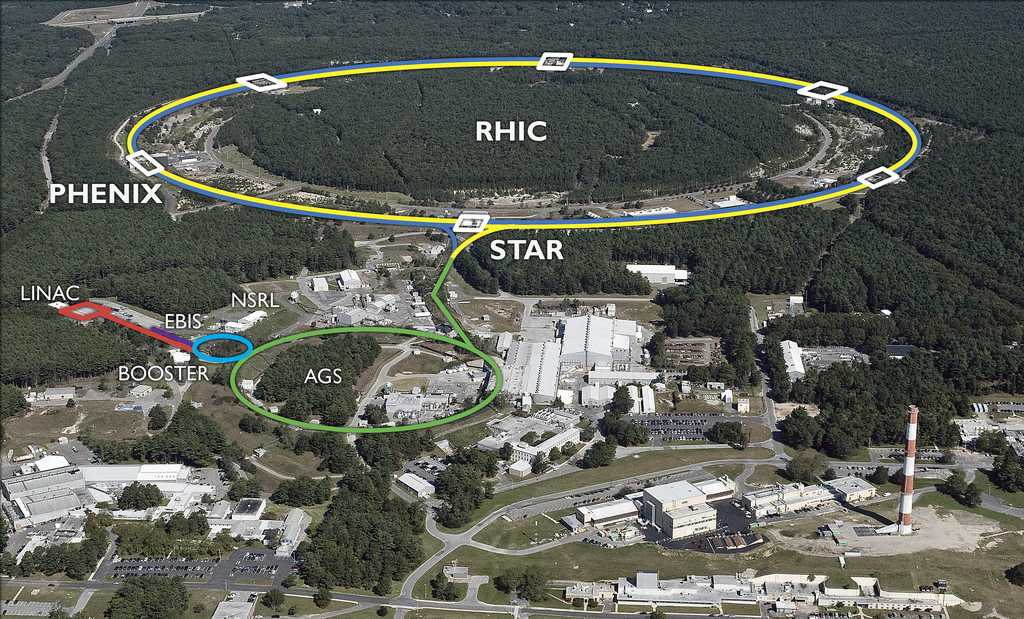
\includegraphics[width=0.6\textwidth]{Figures/RHIC-aerial-HR.jpg}
    \rule{35em}{0.5pt}
  \caption[An Aerial view of BNL]{An Aerial view of BNL with RHIC and the AGS outlined and the locations of PHENIX and STAR mapped}
  \label{fig:Aerial RHIC}
\end{figure}
\indent Based at Brookhaven National Lab (BNL) (Figure \ref{fig:Aerial RHIC}) on the east end of Long Island, New York, the Relativistic Heavy Ion Collider (RHIC) is a particle accelerator and storage ring that is used to study the properties of nuclear matter. Specifically, it is used to observe the properties and formation of the new state of matter, the QGP, formed by nuclear material at extreme temperature and pressure. RHIC accelerates nuclei which are stripped of their electrons (heavy ions) to energies of up to 200 GeV per nucleon, after which the nuclei are steered to collide together with enough energy to raise the system to extremes of pressure and temperature.

\section{The Particle Acceleration Process}
\begin{figure}[htbp]
  \centering
    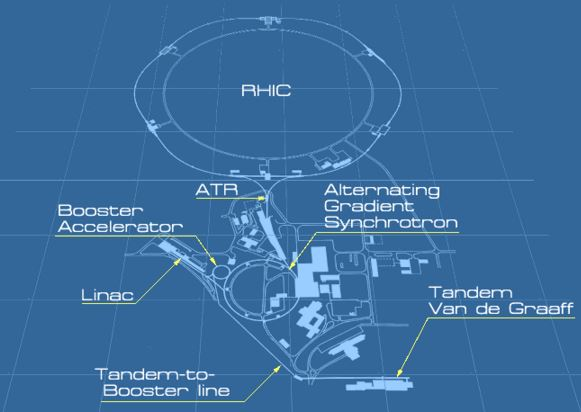
\includegraphics[width=0.8\textwidth]{Figures/RHICdiagram.JPG}
    \rule{35em}{0.5pt}
  \caption[Illustration of all the accelerators used to boost ions to relativistic speeds at RHIC]{Illustration of all the smaller accelerators which are used together in order to boost ions to relativistic speeds at RHIC}
  \label{fig:RHICdiagram}
\end{figure}
The speeds achieved at RHIC are the result of many smaller accelerators working in concert in order to boost the ions' speed increasingly faster \citep{RHICaccel}.  Ions begin their journey at a compact source and heavy ion accelerator called the Electron Beam Ion Source (EBIS) (located by the Linear Accelerator (LINAC) in Figure \ref{fig:RHICdiagram}). From there they are transferred to a circular accelerator called the \textit{Booster Synchrotron} which utilizes long-wavelength radio frequency electromagnetic waves, allowing the ions to ``surf'' on their downward slope. The ions are then fed into the Alternating Gradient Synchrotron (AGS). The AGS was once the proverbial end-of-the-line where the experiments were conducted and studies took place. It is responsible for three Nobel Prizes itself: the discovery of the muon neutrino in 1962, the discovery of charge-parity violation in 1963 (awarded in 1980), and the joint discovery of the J/$\Psi$ in 1976. The AGS uses the alternating fields of 240 magnets in order to focus and boost the ions to 99.7$\%$ the speed of light, after which it is transferred to the \textit{AGS-to-RHIC} transfer line (AtR). The AtR is like a train switchyard wherein bunches of ions are fed into the RHIC rings. These ion bunches are sent through either clockwise in one ring or counterclockwise in the other using a switching magnet.

RHIC is comprised of two concentric rings which are 3.8 kilometers in circumference.  These rings use 1,740 helium cooled superconducting magnets to hold beams of these heavy ions which circulate in opposite directions within the two rings.  Along the circumference of RHIC there are six points where the counter-circulating beams can be steered to collide (Interaction Regions or IR). Of these six IR, four house different detectors: the smaller PHOBOS and BRAHMS experiments, and the larger PHENIX and STAR experiments.  

RHIC is a flexible machine capable of colliding various species of nuclei from protons to uranium \citep{EBISupgrade} over a wide range of energies.  Heavy ions such as Au can be accelerated as low as 3.85 GeV/nucleon and as high as 100 GeV/nucleon \citep{RHIClum}, with a combined center of mass energy of 200 GeV/nucleon.  When accelerating protons, RHIC is able to reach up to 250 GeV since the mass/charge ratio is smaller, and is able to do so with spin-polarized beams. It is also able to do this asymmetrically, that is to say, with two different species of nuclei, one in each ring.  The system studied in this thesis is one such asymmetric system wherein a deuteron is collided with a gold ion with a center of mass energy of 200 GeV/nucleon (this system is referred to as ``d+Au'' in shorthand).

\section{The PHENIX Detector}

\indent The analysis described in this thesis was made using the PHENIX detector which stands for \textit{\textbf{P}ioneering \textbf{H}igh \textbf{E}nergy \textbf{N}uclear \textbf{I}nteraction e\textbf{X}periment}. PHENIX is the largest of the experiments at RHIC and was designed specifically to study the QGP using a wide variety of particle probes at a very high rate with high accuracy.  
\begin{figure}[htbp]
  \centering    
    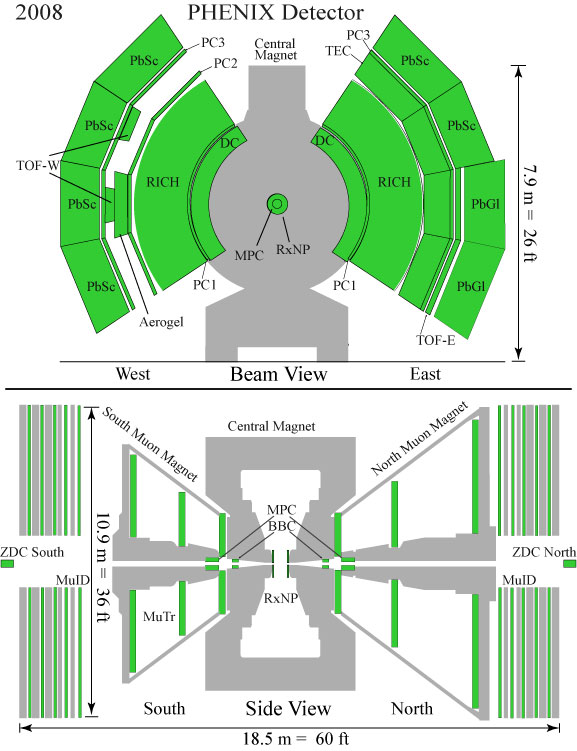
\includegraphics[width=0.8\textwidth]{Figures/Phenix_2008.jpg}
\rule{35em}{0.5pt}
  \caption[PHENIX Detector Configuration for RHIC Run 8 (2008)]{The configuration of the PHENIX detector for Run 8 (2008). The diagram labeled \textit{Beam View} shows the East and West Central Arm spectrometers. In this picture the ion beams would travel into or out of the page through a hole in the center of the region MPC detector. The \textit{Side View} shows the North and South Muon Arms and the location of event characterization detectors such as the ZDC, BBC and RXNP.}
  \label{fig:run8config}
\end{figure}
It consists of a collection of various detectors assembled into four spectrometers called \textit{arms} (see Figure \ref{fig:run8config}). The muon arms are used for studying physics phenomena at forward rapidity\footnote{See Appendix \ref{app:coordinates} for discussion on rapidity.} ($\eta$ = $|1.1-2.4|$). \citep{rapidityref} The system of detectors used for the reconstruction of event tracks of import for this analysis are contained in the \textit{Central Arm}. Accompanying the Central and Muon Arms is a magnet system called the \textit{Central Magnet} and \textit{North and South Muon Magnets} according to their location in PHENIX. The Central Magnet is an axially symmetric field around the beam axis generated by two pairs of Helmholtz coils. The coils are operated independently and are able to be run in various configurations of positive and negative orientation in order to determine systematics \citep{rolnickthesis}. A plot of the field strength vs radius for different configurations of the central magnet is shown in Figure \ref{fig:centralmagnet}.

\begin{figure}[htbp]
  \centering
    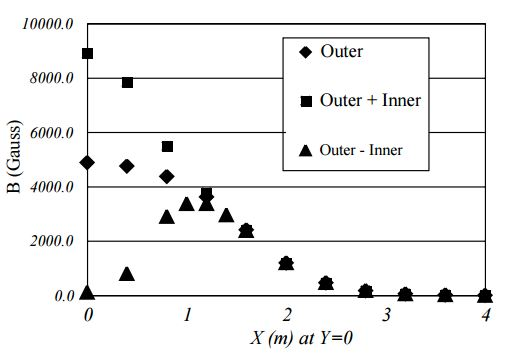
\includegraphics[width=0.6\textwidth]{Figures/phenixcentralmagnet.JPG}
      \rule{35em}{0.5pt}
  \caption[PHENIX Central Magnet Field Strengths.]{PHENIX Central Magnet Field Strengths for different polarities of inner coils vs radial distance from center of IR}
  \label{fig:centralmagnet}

\end{figure}
\subsection{Central Arm}
Covering a rapidity range of $\eta$ $\leq|0.375|$, the Central Arm consists of an East and a West Arm that each cover $90^{\circ}$ azimuthally \citep{EMCfocus} and is a complex, multi-layered, multi-system spectrometer capable of measuring a variety of particle probes. The Central Arm is shown in Figure \ref{fig:run8config} as its individual subsystem detectors highlighted in green\footnote{With the exception of the MPC and RxNP which are not part of the Central Arms, but are in the Muon Arms.}. No single device is ideal for measuring every aspect of a collision event, and, as such, different device technologies that are ideal for measuring specific quantities can be used in concert to gather clean and precise data. In this section the various individual detectors in the Central Arm used in this analysis are discussed.

\subsubsection{Drift and Pad Chambers}
\label{sect:dcpc}
Particle trajectories are tracked using the Drift Chamber (DC) and the Pad Chambers (PC 1,2, and 3) \citep{DCfocus} (labeled DC, PC1, PC2, and PC3 in Figure \ref{fig:run8config}). The DC is a multiwire jet-type drift chamber located between 2.02 and 2.48 m radially from the interaction point, constructed from 6 modules comprised of networks of wires or \textit{nets} in each arm. In principle the DC is similar to a wire chamber; when a charged particle travels through the gas in the DC, the gas atoms are ionized and these electrons and ions are accelerated to anode and cathode wires, respectively, which collect this ionization and send a signal proportional to the ionization effect of the traveling particle. The DC is filled with a gas that is selected to have a uniform drift velocity close to the anode wires, i.e., a gas where the ions and electrons created by outgoing charged particles have a linear relation in position and time such that $x(t) = v_{drift} * t$ within the active region. The gas chosen is a mixture of equal parts argon and ethane, also chosen for the mixture's high gas gain amplification and low diffusion coefficient. The wire nets in the DC are arranged in different predetermined ways with respect to the beam axis. The six modules containing the wire nets are designated names: X1, U1, V1, X2, U2, and V2 (see Figure \ref{fig:dcdiagram}). There are twelve anode wires in each X net and the wires are configured to be parallel to the beam axis so that they can be used to measure the azimuthal angle, $\phi$. The U and V nets are stereo pairs with four anode wires in each net and are tilted by an angle of 4.5$^\circ$ with respect to the beam axis. This angular bias allows for measurement of the track's z-component with high resolution. Furthermore, all wire nets are oriented in layers radially such that outgoing tracks deposit linear, correlatable signals in the DC. Additionally, since the DC is the first detector subsystem that outgoing particles created in a collision pass through, it is also used in conjunction with other detectors in order to accurately determine track trajectory through all of the detectors in the central arm. The method of track reconstruction will be discussed in Section \ref{trkrecosect}.

\begin{figure}
  \centering
\begin{subfigure}[p]{1\textwidth}
  \centering
    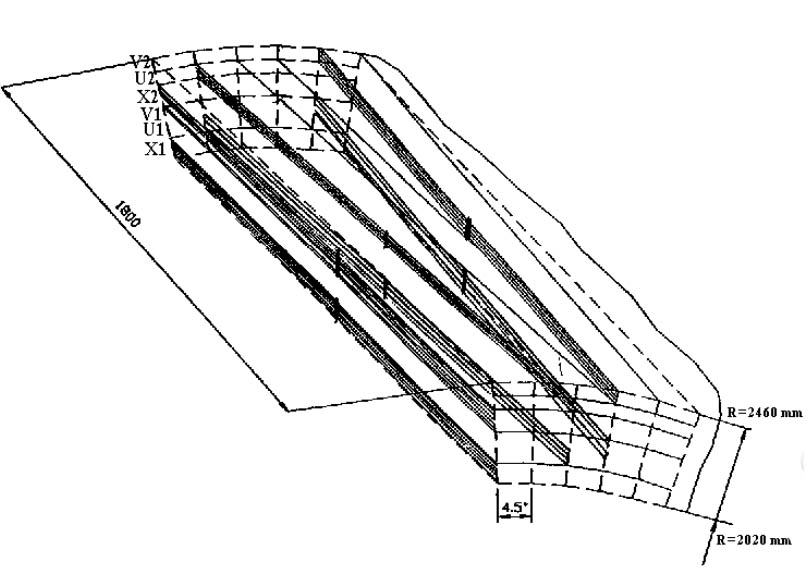
\includegraphics[width=1\textwidth]{Figures/dcdiagram.jpg}
  \caption{A diagram showing the radial configuration of the various wire nets in the DC. The X1 plane is the innermost radius DC wire network, followed by the stereo pair U1 and V1, X1, and another stereo UV pair.}
  \label{fig:radialdcdiagram}
\end{subfigure}
\end{figure}
\begin{figure}
    \ContinuedFloat % continue from previous page
\begin{subfigure}[p]{1\textwidth}
  \centering
    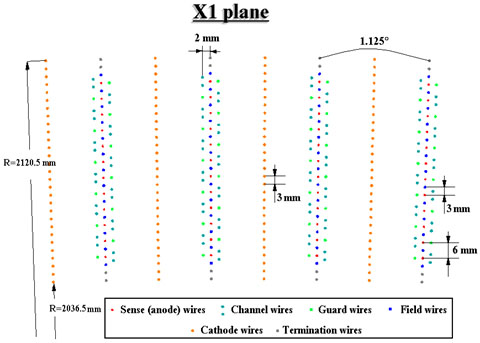
\includegraphics[width=1\textwidth]{Figures/DCX1net.jpg}

  \caption{The radial configuration the X-type wire nets in the X1 plane. Each X-type wire net consists of twelve anode wires.}
  \label{fig:X1dcdiagram}
\end{subfigure}

\begin{subfigure}[p]{1\textwidth}
  \centering
    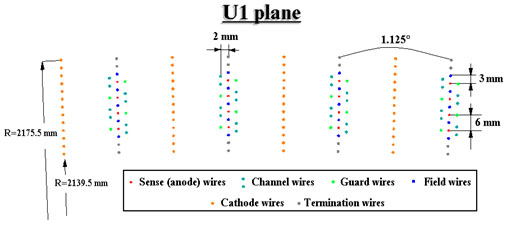
\includegraphics[width=1\textwidth]{Figures/DCU1net.jpg}
    
  \caption{The radial configuration the U-type (and V-type) wire nets in the U1 plane. Each U-type wire net consists of four anode wires and are paired with a radially following identical V-type wire net.}
  \label{fig:U1dcdiagram}
\end{subfigure}
\rule{35em}{0.5pt}
\caption[Diagrams of DC wire configurations.]{Diagrams of DC wire configurations.}
\label{fig:dcdiagram}
\end{figure}
The Pad Chambers \citep{PCfocus} (PC) are three individual layers of pixel detectors. The PCs have the same azimuthal coverage as the DC and the rest of the Central Arm and are located at increasing concentric distances from the collision vertex, the DC being the inner most detector, followed immediately by PC1\footnote{Located 2.5 m radially from nominal IR.} (see Figure \ref{fig:pcdiagram}). PC2\footnote{Located 4.2 m radially from nominal IR.} only exists in the west arm however PC3\footnote{Located 4.9 m radially from nominal IR.} exists in both arms. The pixels in these detectors are arranged into nine pixel clusters called ``pads'' which are read out by a single channel. The pads in the innermost radius PC (PC1) are 8.4 mm x 8.45 mm and the pads in PC2 and PC3 are sized to maintain the same angular resolution at further radial distances. The small size of the individual pads allows for a large pixel density which is important for maintaining the separation of individual track signals in a high luminosity, high multiplicity event such as that of central heavy ion collisions. Since these detectors can be used to accurately determine particle track trajectories, and since charged particle trajectories curve under the influence of a magnetic field, the track curvature can be used to determine the particle's momentum. This track location data is also used to match with other detector data such as calorimetry, time of flight, and Cherenkov counters.
\begin{figure}[htbp]
  \centering
    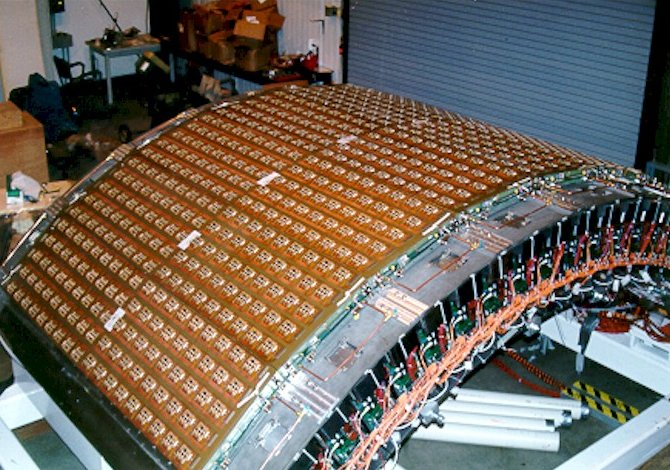
\includegraphics[width=0.7\textwidth]{Figures/PC1.jpg}
    \rule{35em}{0.5pt}
  \caption[Pad Chamber 1 on top of the Drift Chamber.]{Pad Chamber 1 on top of the Drift Chamber.}
  \label{fig:pcdiagram}
\end{figure}

\subsubsection{TOF: Time Of Flight Detectors}

In addition to the tracking detectors, this analysis utilizes high accuracy Time of Flight (TOF) detectors that are used to measure the time it takes for charged particles traveling through the Central Arm to go from the event vertex to the detector. \citep{TOFfocus} There are two TOF detectors in PHENIX, one on the East Arm and one on the West Arm. Located five meters away from the collision vertex and in the lower two sectors of the east arm (see Figure \ref{fig:run8config}) the TOF East (TOFE) is a scintillation detector with a timing resolution of $\Delta t_{res} \leq 100 ps$. It covers $\Delta\phi = \pi / 4$ and $\eta < |0.35|$. 

\begin{figure}[htbp]
  \centering
    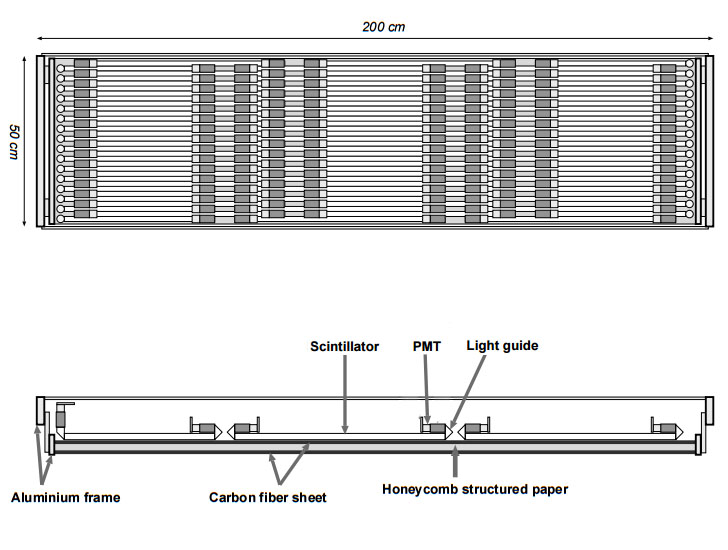
\includegraphics[width=0.8\textwidth]{Figures/TOFEschematic.jpg}
    \rule{35em}{0.5pt}
  \caption[A schematic of the slat layout in the TOFE.]{A schematic of the slat layout in the TOFE. The top figure depicts the slat layout facing the IR, the bottom figure is a side view of the slats showing the configuration of the subparts of each slat.}
  \label{fig:TOFEschematic}
\end{figure}

Scintillators are a special type of material that fluoresces when hit by a charged particle or high-energy photon. The TOFE is comprised of 1000 15.1 mm "slats" of plastic scintillation material with two photomultiplier tubes (PMT) on either end of the slats (see Figure \ref{fig:TOFEschematic}). These PMTs are devices that utilize the photoelectric effect to translate photons generated in the scintillator into an electric signal. The strength of this signal is often proportional to the number of electrons generated by the photons incident on the PMT, hence they are called photoelectrons. Since we know the length of the slat and the speed of light in the scintillation material we can easily calculate both the time when the particle first hit the slat ($T_{0}$) and the position where the particle hit the slat ($y$),
\begin{equation}
T_{0} = \frac{(T_{1}+T_{2})-L/v}{2} , \, \, y = \frac{T_{1}-T_{2}}{2} v
\end{equation}
where $T_1$ and $T_{2}$ are the times measured by PMTs 1 and 2 relative to the event start time measured by the BBC (see Section \ref{sect:timeandvtx}), $L$ is the length of the slat, and $v$ is the speed of light in the scintillator.

\begin{figure}[htbp]
  \centering
    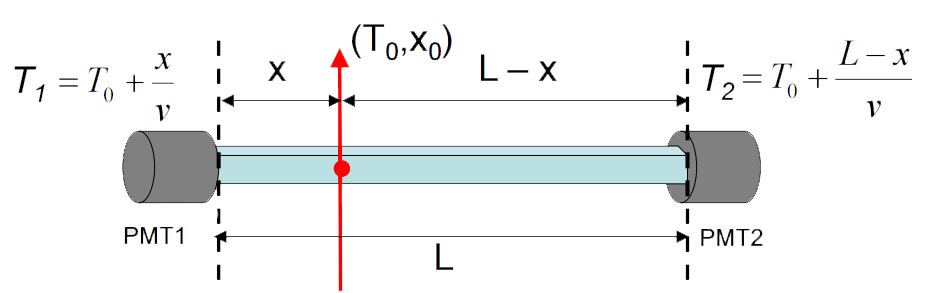
\includegraphics[width=0.8\textwidth]{Figures/TOFEcartoon.jpg}
    \rule{35em}{0.5pt}
  \caption[An illustration of a single slat in the TOFE.]{An illustration of a single slat in the TOFE.}
  \label{fig:TOFEcartoon}
\end{figure}

In the West Arm, the TOF West (TOFW) is a 1024 channel Multi-gap Resistive Plate Chamber (MRPC) detector with a timing resolution of $\Delta t_{res} < 100 ps$, located 4.85 m from the collision vertex and also covering $\Delta\phi = \pi / 4$ and $\eta < |0.35|$. The MRPC works on the same general principle as a basic Resistive Plate Chamber (RPC) which is comprised of two high resistivity plates separated by a volume of gas. On one resistive plate is a sheet of conducting material that is used to maintain a constant electric field across the gas gap. The other resistive plate has an array of conducting readout strips. When a charged particle travels through the gas it causes an electron-ion avalanche similar to what happens in a drift chamber. The electron avalanche is accelerated under the influence of an externally applied electric field toward one of the readout strips resulting in a ``hit'' signal which is then amplified by electronics. 

\begin{figure}[h]
  \centering
    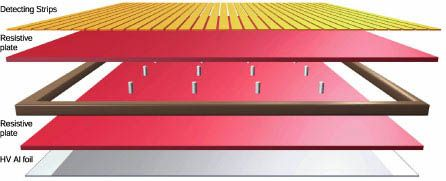
\includegraphics[width=0.8\textwidth]{Figures/RPClayers.jpg}
    \rule{35em}{0.5pt}
  \caption[Diagram of a basic RPC.]{Diagram of a basic RPC \citep{CMSRPC}.}
  \label{fig:RPCbasic}
\end{figure}

A MRPC is a version of an RPC with alternating layers of the resistive material and gas gaps sandwiched together with the high voltage surface and readout strips on the outermost sides of the device \citep{Akindinov:2000rq} (see Figure \ref{fig:RPCbasic}). The resistive plates inside the sandwich are electrically isolated and are transparent to the fast signals of incoming particles. An externally applied electric field induces charges on the surfaces of the resistive plates, causing each of the small gas gaps to be held at the same potential. Like the basic RPC design, incoming particles ionize the gas causing an avalanche of electrons and ions in each of the gas gaps and an electric signal is deposited on the readout strips. The total signal the strips see is the \textit{sum} of all of the electrical activity in each of small gaps. By using this configuration of small parallel uniform gaps, a greater precision is allowed than conventional RPC designs, which lends itself well to high precision timing detectors.

\begin{figure}[ht!]
  \centering
    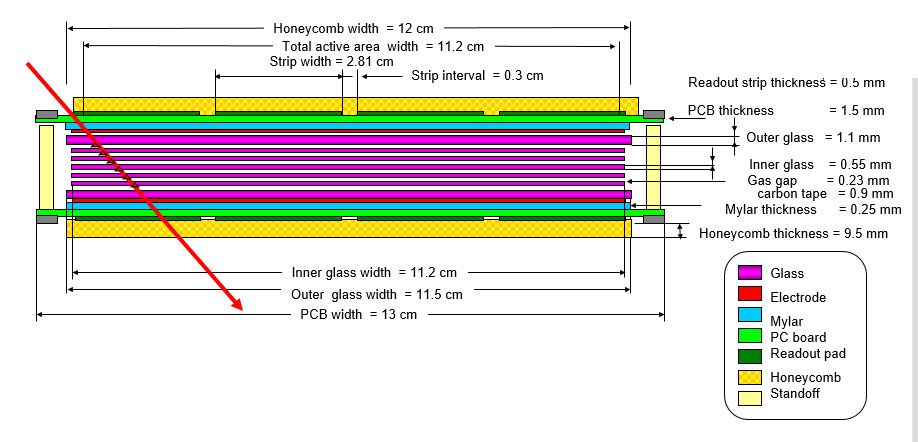
\includegraphics[width=0.8\textwidth]{Figures/MRPC_TOFW.jpg}
    \rule{35em}{0.5pt}
  \caption[Cross sectional diagram of the MRPCs used in the TOFW.]{Cross sectional diagram of the MRPCs used in the TOFW.}
  \label{fig:MRPCTOFW}
\end{figure}

\subsubsection{ACC: Aerogel Cherenkov Counter}
As measured track momentum increases, the timing resolution of the TOF detectors causes larger uncertainty in the timing measurements which, in turn, leads to a larger uncertainty in the particle mass. This uncertainty broadens the Gaussian-shaped particle mass distribution, gradually causing individual mass distributions to overlap, and eventually become inseparable, as $p_T$ increases. The high resolution capabilities of the TOF detectors only allow them to separate $\pi^{\pm}$, $K^{\pm}$, and $p$ / $\bar{p}$ signals up to certain transverse momentum $p_{T}$ thresholds ($\pi/K$ separation becomes difficult above $p_T$ = 2.1 GeV/c impossible above 2.8 GeV/c, K/p separation is possible only up to 4 GeV/c). The distinct masses of the particles of interest do provide an additional method of separating particle signals, since two particles of different mass with the same momentum have distinct velocities. This is the principle with which a Cherenkov detector works. Cherenkov radiation is light that is emitted in a material when a charged particle travels through it with a velocity faster than the speed of light in that medium. This medium, called a Cherenkov radiator, can be carefully selected such that its intrinsic speed of light is such that lighter particles with higher velocities cause Cherenkov radiation but heavier particles which travel slower given the same momentum will not. This threshold is given by

\begin{equation}
E_{threshold} = \frac{nm}{\sqrt{n^2-1}}
\end{equation}
where \textit{n} is the index of refraction in the Cherenkov radiator and \textit{m} is the mass of the particle.

Using this, a Cherenkov detector acts as a logic detector categorizing tracks as those that either ``fire'' or ``veto'', that is to say tracks that radiate versus tracks that don't. In the case of separating $\pi^{\pm}$ mesons from $K^{\pm}$ mesons for $p_{T}$ tracks where their mass signals overlap so strongly that they cannot be uncorrelated, the radiator was chosen such that the pions will radiate in the detector, but the kaons will not. Pions and kaons are indistinguishable for $p_{T} > 2.8$ GeV/c, so the radiator chosen to separate the signals is a silica aerogel ($n \approx 1.011$).

The Aerogel Cherenkov Counter (ACC) is comprised of 160 tiles of silica aerogel. Each tile is affixed to a cube which forces radiated Cherenkov photons to reflect internally until they hit a PMT (see Figure \ref{fig:accchannel}). These cubes are filled with air and are covered on all exposed sides by a Gore-Tex reflector except for the ``front'' facing aerogel tile side and the two cutouts where the PMTs attach. Due to the fact that the cube uses internal reflection to maximize the number of photons collected by the PMTs it is called an integration cube. There are two PMTs located opposite from each other for each cube. To account for the space taken by PMTs on the ends of the tiles, the ACC is two sided and the tiles are oriented such that the opposite side tile occupies the gap where PMTs would be situated (this configuration can be seen on the ``Top View'' labeled diagram on Figure \ref{fig:ACCschematic}). There are ten rows of eight tiles on each side for a total of 160 tiles.

The ACC is located in the west arm covering the half of the azimuthal coverage that the TOFW covers and with the same rapidity coverage (see Figure \ref{fig:run8config}). When used in conjunction with the TOFW, it can provide pion/kaon separation for $p_{T} < 4$ GeV/c and can discriminate protons for $p_{T} < 7$ GeV/c.  The total particle identification capabilities of the combination of the TOFW + ACC is shown in Figure \ref{fig:PIDrange}.

\begin{figure}
\begin{subfigure}[p]{1\textwidth}
   \centering
    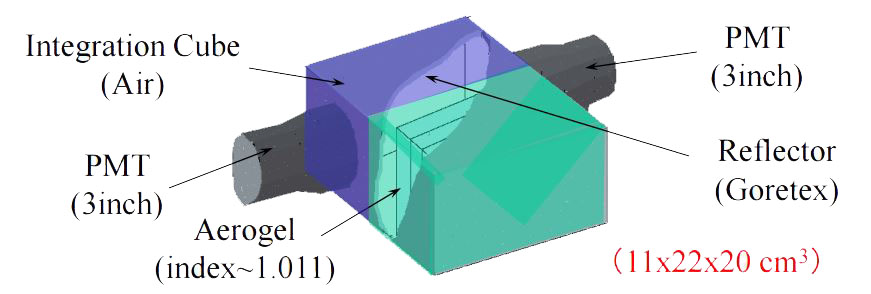
\includegraphics[width=0.8\textwidth]{Figures/aerogelchannel.JPG}
  \caption[A schematic of one tile in the ACC]{A schematic of one tile in the ACC}
  \label{fig:accchannel}
    \rule{35em}{0.5pt}\end{subfigure}
\begin{subfigure}[p]{1\textwidth}
  \centering
    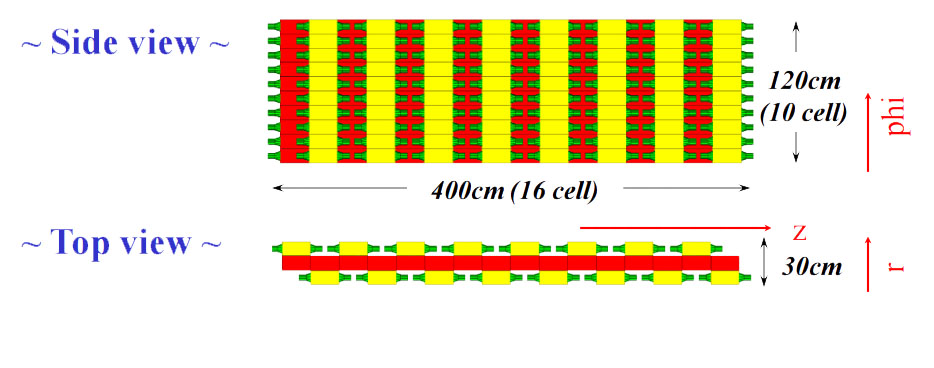
\includegraphics[width=0.8\textwidth]{Figures/ACCschematic.jpg}

  \caption[A schematic of the Aerogel Cherenkov Counter]{A schematic of the layout of the Aerogel Cherenkov Counter. Yellow boxes represent Aerogel tiles and integration cubes. Green cylinders on either end of the yellow boxes are the PMTs.}
    \rule{35em}{0.5pt}
  \label{fig:ACCschematic}
\end{subfigure}
\begin{subfigure}[p]{1\textwidth}
  \centering
    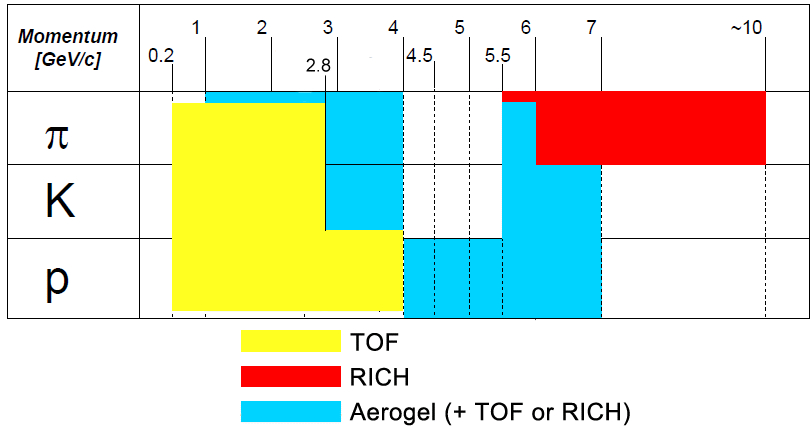
\includegraphics[width=0.8\textwidth]{Figures/accrange.jpg}
  \caption[Chart of Particle Identification capabilities over a range of transverse momentum.]{Chart of Particle Identification capabilities over a range of transverse momentum with combinations of detectors.}
    \rule{35em}{0.5pt}
  \label{fig:PIDrange}
\end{subfigure}
\caption{}
\end{figure}


\subsubsection{EMCal and RICH: Electromagnetic Calorimeter and Ring Imaging Cherenkov Counter}
Two other detectors that provide important track data are the \textit{Electromagnetic Calorimeter} (EMCal) and the \textit{Ring Imaging Cherenkov Counter} (RICH). Each arm has full coverage with both the RICH and the EMCal and they are often used together in order to study electrons via the EMCal/RICH Trigger (ERT). For the scope of this analysis, only the RICH is used in order to reject electron tracks which can contaminate the pion signal; the EMCal will be discussed for completeness.

As evident from its name, the RICH (Figure \ref{fig:RICHdiagram}) is a Cherenkov counter that is used in a similar fashion as the ACC, namely, to discriminate between particle species using Cherenkov radiation as a logic trigger. In the case of RICH, we are interested in separating pion and electron signals. It is filled with CO$_2$, which was chosen because it would allow electrons to radiate at very low $p_T$ ($>$ 0.018 GeV/c) while pions would not until the relatively high $p_T$ of 4.87 GeV/c. Cherenkov radiated photons are emitted parallel to each other along the track path as electrons move through the detector. The outer surface of the RICH is a series of mirrors arranged to form a spherical mirror which focuses that Cherenkov light onto the 2560 PMTs/arm which line the inner surface of the RICH. This results in a ring shaped Cherenkov signature as measured by the PMTs, hence the name: Ring Imaging Cherenkov Counter. 

\begin{figure}[h!]
  \centering
    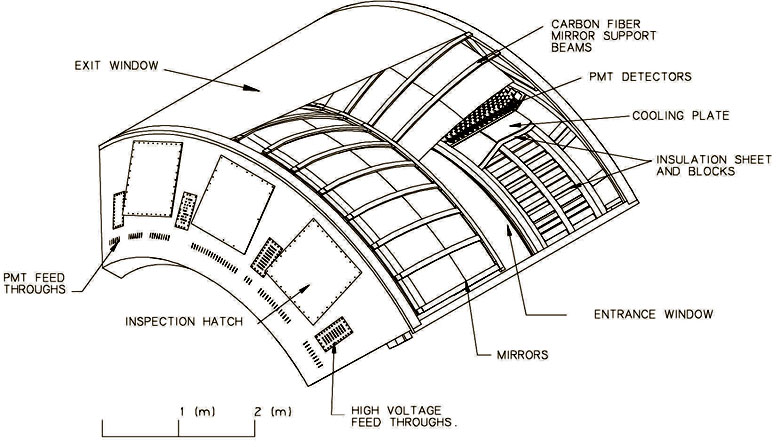
\includegraphics[width=0.8\textwidth]{Figures/RICHdiagram.jpg}
    \rule{35em}{0.5pt}
  \caption[A diagram of the RICH]{A diagram of the RICH}
  \label{fig:RICHdiagram}
\end{figure}

\begin{figure}
\centering
\begin{subfigure}[p]{0.5\textwidth}
    \centering
    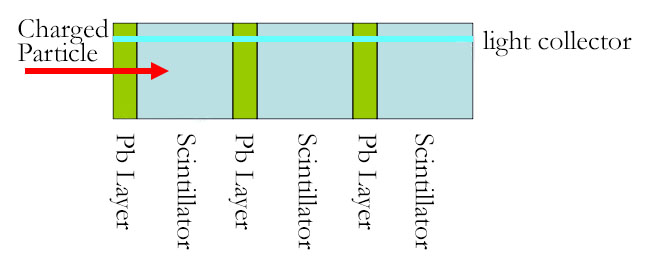
\includegraphics[width=\textwidth]{Figures/PbScschematic.jpg}\ssp
    \caption{Schematic of a PbSc module. Pb layers cause EM showers which create light in the scintillators and are detected by the light collectors.}
\label{fig:pbsc}
\end{subfigure}
\begin{subfigure}[b]{0.6\textwidth}
    \centering
    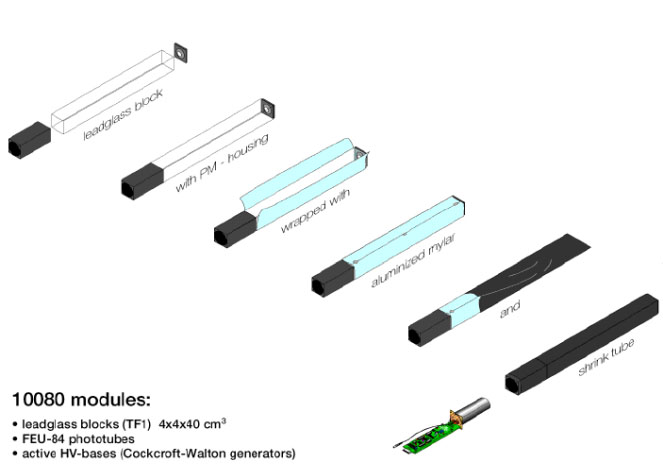
\includegraphics[width=\textwidth]{Figures/PbGlmodules.jpg}
    \caption{Construction of PbGl modules.}
\label{fig:pbglmodule}
\end{subfigure}
\begin{subfigure}[b]{0.6\textwidth}
    \centering
    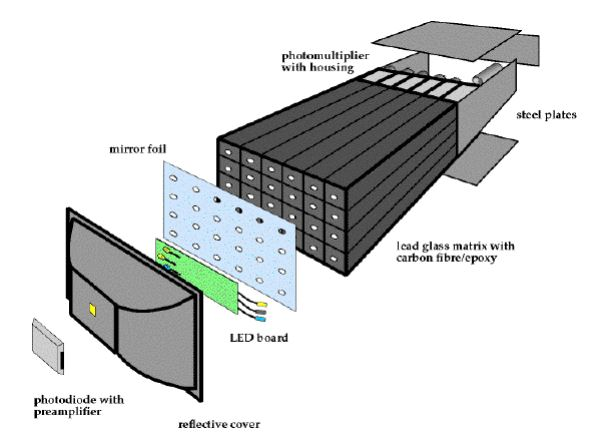
\includegraphics[width=\textwidth]{Figures/pbglsupermodule.JPG}
    \caption{One PbGl super module.}
\label{fig:pbglsupmodule}
\end{subfigure}
\rule{35em}{0.5pt}
\caption[Schematics of EMCal components.]{Schematics of EMCal components.}
\label{fig:EMCalcomponents}
\end{figure}
\dsp

The EMCal measures the energy of charged particles and is broken up into eight sectors, with four sectors in each arm \citep{EMCfocus}. Six of the sectors (all four of the west arm and the top two in the east arm) are made of channels comprised of alternating layers of lead and scintillator (PbSc) material (fig \ref{fig:pbsc}). The lead layers cause incoming particles to shower into the scintillator layers that generate light which is detected by PMTs. The lower two sectors in the East Arm are comprised of 10,080 uniform lead glass Cherenkov radiator towers (PbGl) (Figures \ref{fig:pbglmodule} and \ref{fig:pbglsupmodule}). These towers have PMTs attached on one end and are wrapped individually in reflective Mylar and shrink wrapped to form \textit{modules}. They are then placed in grid-like networks and each 16 module x 12 module structure is read out by one photodiode/preamplifier combination. 

Two types of detector are used in the EMCal because they each have their own strengths. PbSc is more linear in response and is better at timing than PbGl thanks to its alternating layers, whereas PbGl is a tried-and-true design used in previous experiments such as WA98 at the SPS at CERN for its exceptional granularity and accurate energy measurement. Because they are two separate systems, they have different systematics, and, therefore, we have a higher confidence level for the physics results from the EMCal. 

%As mentioned, the EMCal and RICH are used together to form a level 1 trigger to classify charged tracks. Since the RICH is tuned to radiate with electron tracks and the EMCal measures all charged tracks, we know that tracks that result in signals in both the EMCal and the RICH are most likely electrons, whereas tracks that only have signals in the EMCal are likely charged hadrons (fig \ref{fig:ERT}).
%\begin{figure}[h!]
%  \centering
%    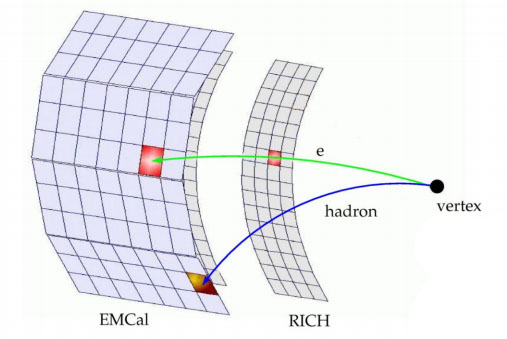
\includegraphics[width=0.5\textwidth]{Figures/ERT.jpg}
%    \rule{35em}{0.5pt}
%  \caption[A drawing of ERT event discrimination.]{A drawing of ERT event discrimination.}
%  \label{fig:ERT}
%\end{figure}

\subsection{Forward and Global Detectors}
Though the bulk of this analysis is dependent on the central arm detectors, many aspects of reconstruction, namely event characterizations (start of the event timer, the event vertex, centrality, and event reaction plane), are dependent on a handful of forward-rapidity detectors which will be briefly discussed here.

\subsubsection{BBC: Beam-Beam Counter}
Of the forward detectors, the \textit{Beam-Beam Counter} (BBC) \citep{BBCfocus} is probably the most important because of its ability to measure the various global event parameters. There are two BBCs, one on the north side and one on the south side of PHENIX both equidistant (144 cm) from the center of the interaction region (IR). The constituent detector (Figure \ref{fig:BBCillustrations}) elements are made of quartz Cherenkov radiators attached to meshed dynode PMTs housed in hexagonal encasements. These elements are arranged in a toroidal shape (inner and outer radii of 5 cm and 30 cm respectively) in order to allow the ion beams to pass through the center while still getting full $2\pi$ azimuthal coverage. The BBCs cover 3.1$\leq \Delta \eta \leq$4 in pseudorapidity. 
\begin{figure}
\centering
\begin{subfigure}[b]{0.4\textwidth}
    \centering
    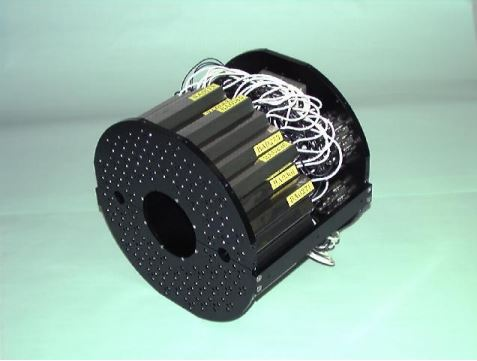
\includegraphics[width=\textwidth]{Figures/bbcrender.JPG}
    \caption{An illustration of a BBC.}
\end{subfigure}
\begin{subfigure}[b]{0.4\textwidth}
    \centering
    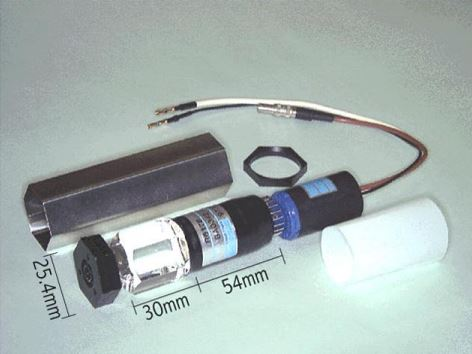
\includegraphics[width=\textwidth]{Figures/bbcsinglechannel.JPG} 
    \caption{A single element of the BBC.}

\end{subfigure}
 \rule{35em}{0.5pt}
\caption[The Beam Beam Counter.]{The Beam Beam Counter.}
    \label{fig:BBCillustrations}
\end{figure}

\subsubsection{ZDC/SMD: Zero Degree Calorimeter and Shower Max Detectors}
\label{sect:ZDC}

\begin{figure}

\begin{subfigure}[p]{1\textwidth}
  \centering
    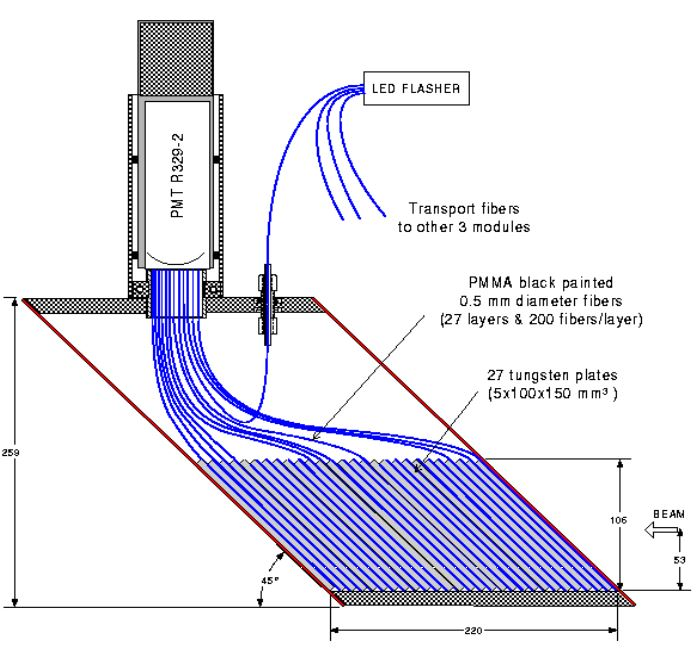
\includegraphics[width=0.5\textwidth]{Figures/ZDCschematic.JPG}

  \caption[Schematic showing a side view of the layout of fiber optics in the ZDC]{Schematic showing the layout of fiber optic ribbons in the ZDC.}
  \label{fig:zdcschem}
   \rule{35em}{0.7pt}
\end{subfigure}
\begin{subfigure}[p]{1\textwidth}
  \centering
    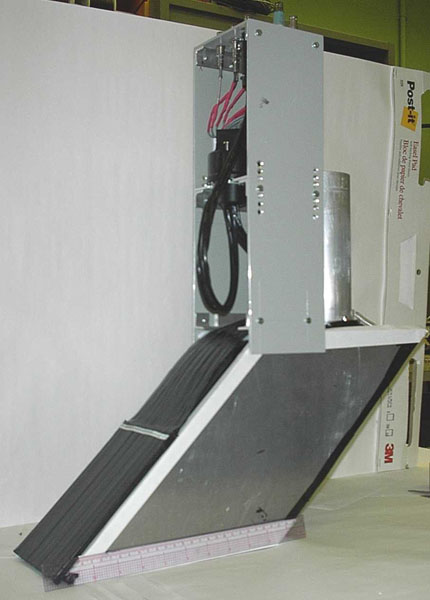
\includegraphics[width=0.4\textwidth]{Figures/SMDonZDC.jpg}

  \caption[Picture of the SMD.]{A picture of an SMD. 21 scintillators resting on top of a ZDC module. Another ZDC module will go in front of this. The beam would hit from the lower left going right if this were installed in the beam pipe like this.}
  \label{fig:smdonzdc}
   \rule{35em}{0.7pt}
\end{subfigure}
\caption{The ZDC and SMD.}
\end{figure}

Crucial to the determination of event centrality is the ability to count the number of spectator particles. Since neutrons have no charge, we can place a calorimeter at high rapidity behind an IR dipole magnet (18 m away from the nominal event vertex) which we can use to ``sweep'' away charged particles like proton spectators and other charged track noise (see ``Side View'' on Figure \ref{fig:run8config}). The \textit{Zero Degree Calorimeter} (ZDC) \citep{ZDCfocus} is comprised of ribbons of acrylic fiber optic strands sandwiched between two tungsten plates (Figure \ref{fig:zdcschem}). The tungsten plates act as a dense absorber for the neutrons to hit and shower into resulting in detectable photon yield in the fiber optic ribbon. There are three ZDC modules on each side of PHENIX. Sandwiched between modules of the ZDC is a hodoscope called the \textit{Shower Max Detector} (SMD) (Figure \ref{fig:smdonzdc}). The SMD is comprised of 21 0.5 cm x 0.5 cm scintillators and is used to measure the centroid of the shower in Cartesian coordinates since the ZDC only measures energy \citep{phenixzdc}. This shower location determination of the SMD makes it useful as another detector with which to determine the \textit{event plane} (see Section \ref{sect:eventplane}. The ZDC is used in conjunction with the BBC in order to determine centrality. Since more peripheral collisions mean more spectators and therefore more neutrons to hit the ZDC, the higher the energy measured by the ZDC the more peripheral the event (see Figure \ref{fig:zdcvsbbc} \citep{Ghosh2001}). 

\subsubsection{MPC: Muon Piston Calorimeter}
The \textit{Muon Piston Calorimeter} (MPC) was a needed upgrade to PHENIX that provided calorimetry at very high rapidity \citep{kleinjanthesis}. It was installed in two parts as follows, first in the south in 2005, then in the north in 2006, and was commissioned to reconstruct $\pi^{0}$ and $\eta$ mesons for various forward physics analyses. Due to its forward location ($3.1 \leq  | \eta | \leq 3.7$ ($3.9$ in the north)) and full azimuthal coverage, it is another detector that is ideal for determining the reaction plane. Nestled in a gap in the piston of the Muon Magnet Arms, the MPC is comprised of lead tungstate $PbWO_4$\footnote{196 in the south, 220 in the north.} crystal scintillator towers attached to avalanche photodiodes with preamplifiers to measure the electromagnetic shower photons as in Figure \ref{fig:mpcschematic}, with its location in PHENIX labeled on Figure \ref{fig:run8config}.  

\begin{figure}[h!]
  \centering
    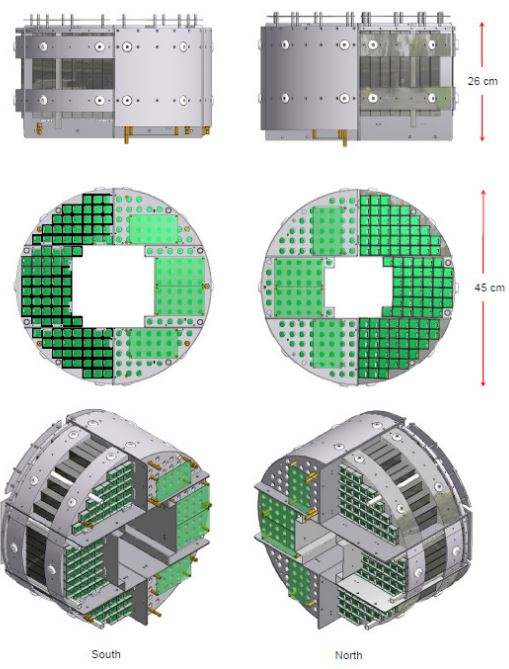
\includegraphics[width=0.7\textwidth]{Figures/mpcschematic.JPG}
    \rule{35em}{0.5pt}
  \caption[Schematic of the MPC]{Schematic of the MPC. The toroidal shape of the tower configuration allows it to nestle inside the piston of the muon arms while allowing ion beams to travel through the center.}
  \label{fig:mpcschematic}
\end{figure}

\subsubsection{RXNP: Reaction Plane Detector}
The \textit{Reaction Plane Detector} (RXNP) is a forward detector subsystem \citep{RXNPfocus} with full azimuthal coverage in 12 segments. It has two segments in rapidity as follows: an inner segment that covers $1.5 \leq \eta \leq 2.8$ and an outer segment that covers $1.0 \leq \eta \leq 1.5$. There are two RXNP detectors, one on each muon arm. All segments are made of 2 cm thick plastic scintillators with a 2 cm layer of lead placed directly in front that acts as a converter, causing all tracks to shower before hitting the scintillators \citep{RXNPfocusER}.  
\begin{figure}
\begin{subfigure}[h]{1\textwidth}
    \centering
    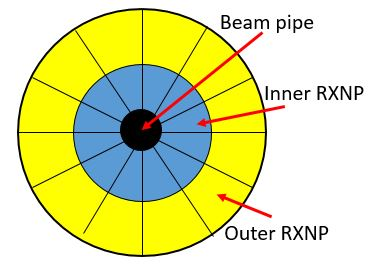
\includegraphics[width=0.5\textwidth]{Figures/RXNPdiagram.JPG}
    \caption{The beam axis view of the RXNP. The blue ring is the inner RXNP, the yellow, the outer RXNP.}

\end{subfigure}
\begin{subfigure}[h]{1\textwidth}
\centering
  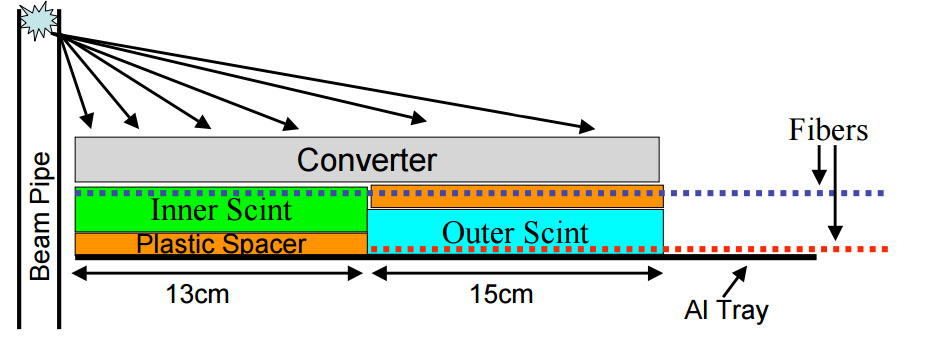
\includegraphics[width=0.7\textwidth]{Figures/RXNPschem.jpg}
  \caption{Cross sectional diagram of RXNP layers. Produced particles hit a lead layer that causes them to shower into the scintillators.}
\end{subfigure}

  \rule{35em}{0.5pt}
\caption[Diagram and picture of the RXNP detector]{Diagram and picture of the RXNP detector}
      \label{fig:RXNP}
\end{figure}

\section{The DAQ}
Each of these detector subsystems capture large amounts of data per event, and the high luminosity of RHIC collisions resulting from millions of events per second doesnt allow the computation systems, reconstruction, or network storage capabilities time to catch up. The process of optimizing collecting data created from a high-event-rate, high track multiplicity experiment, in the form of dozens of event and track variables collected by thousands of individual readout channels in a handful of individual subsystems, all funneled through a single data acquisition system that organizes everything and prepares the data for analysis is an intricate and chaotic symphony \citep{DAQfocus}. In order to do this, the \textit{Data Acquisition} system (DAQ) breaks up the data flow into smaller groups called \textit{partitions} which are assembled from the small collection of data channels called \textit{granules}, typically consisting of sectors of detector subsystems. RHIC is authorized to take data for only a few months out of the year. In practice, this results in three 8 hour manned shifts a day, 7 days a week, for the duration of the run, with data taking only stopping when re-injecting RHIC with ions.

Each granule consists of a \textit{Granule Timing Module} (GTM), a \textit{Front End Module} (FEM), and a \textit{Data Collection Module} (DCM).  The GTM synchronizes with the overall DAQ clock, which is also synchronized with the RHIC clocks. These clocks optimize the amount of time the DAQ is actively processing data (called its \textit{livetime}) so that the DAQ is live when bunches of ions are colliding at a maximum rate. The FEMs take the raw output from the preamplifiers in the individual readout channels of a detector subsystem and organizes them into coherent data packets that are transferred over fiber optics to the DCMs. The DCMs act as a sort of stop light regulating the flow of data into buffers with the GTM clock so that data packets from various subsystems are in sync with each other from the same event as they go into the buffer boxes before being transferred to storage. Even with this timing and granule optimization, RHIC's event rate is so high that it is impossible to collect every track that passes through its subsystems. The process of utilizing real time detector data to discern which events should be kept and what should be rejected is called \textit{triggering}. There are many triggers at different levels of the DAQ, for example the aforementioned ERT is a trigger that allows us to only collect electron events (or vice versa, reject electron events), events that are of interest for dilepton analyses such as Drell-Yan and J/Psi measurements (or to remove electron noise from charged pion analyses such as this one). The master trigger that sets the timing for the whole DAQ is called the \textit{Global Level 1} trigger or the GL1. It synchronizes large track multiplicity signal coincidence collected by the ZDC to the start of the event and checks to see if the buffers in each granule are clear. Other triggers such as \textit{Local Level 1} (LL1) utilize data from the BBCs to ensure the event vertex happens within a region that will result in acceptable track acceptance and scale down the overall event collection rate so that the buffers have time to clear between event data processing cycles.

\begin{figure}[h!]\captionsetup{width=1.1\linewidth}
  \centering
    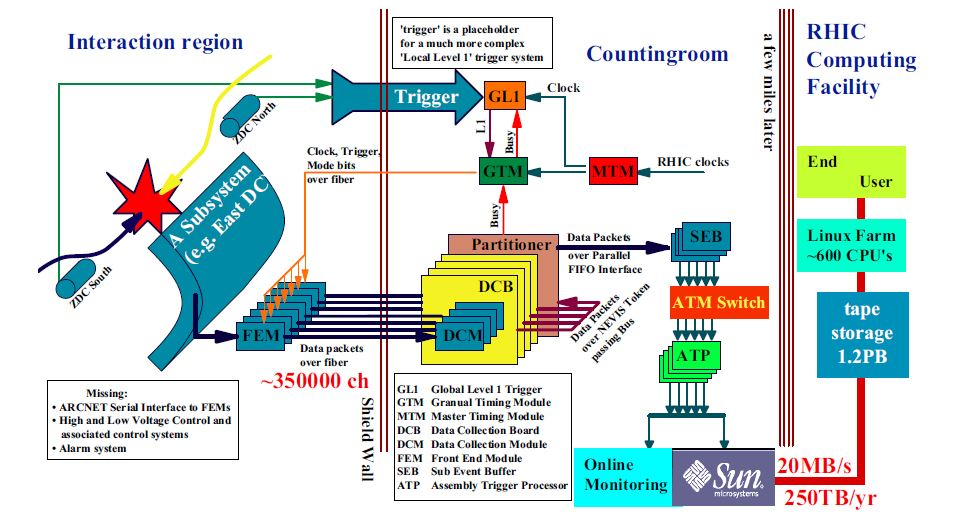
\includegraphics[width=1\textwidth]{Figures/DAQ.jpg}
    \rule{35em}{0.5pt}
  \caption[A diagram of the data flow of PHENIX data through the DAQ]{A flow chart of the data collection, triggering, and processing through PHENIX's DAQ. Collisions happen in the left side of the chart. The ZDCs calculate the start time of the event and tells the Global Level 1 (GL1) trigger that an event has started. Concurrently, particles created in the collision fly out of the IR and deposit track data into detector subsystems. These subsystems send raw analog data to the Front End Modules (FEM) which convert the signals to digital packets of data. This data is sent to Data Collection Modules (DCM) and is associated with a specific collision event via the Granule Timing Modules (GTM) which interface with the GL1. When the GL1 confirms the start of the event, data coming through the DCMs is sent to the Sub Event Buffers (SEB) which throttles the flow of data and stores data short term from all the subsystem granules so that it can all be transferred to the RHIC Computing Facility (RCF) for storage. This last stage of data flow is controlled by the Assembly Trigger Processors (ATP) which not only manages the data flow from the SEBs to RCF but also sends real time diagnostic information about the status of various detector subsystems, buffer size, data rate, etc. to the Control Room (Online Monitoring).}
  \label{fig:DAQ}
\end{figure}

\pagebreak
\pagebreak
